\section{Providing hardware usage accounting}
\label{sec:hw}

%Building on the findings of \cite{pathak2012energy}, who have shown the I/O components to be the energy-greediest, one can already get an insight of the shape of the energy breakdown by hardware component produced by most applications.
%Moreover, many tools, such as \petra{} \cite{petra} or \vlens \cite{li2013calculating}, already aggregate the drain caused by each component and could be easily extended to produce such breakdowns at the source-line granularity.
%However, very few contributions focussed on tail-energy and software-based approaches were never used to this end.
%Therefore, it was our view that this work should first focus on tail-energy accounting for an I/O component, and Wi-Fi was chosen for practical purposes.
%It was then questioned what information representative of the tail-power behaviour should be presented to the user.
%In order to help developers reduce the fraction of energy spent in tail mode, \eprof{} \cite{pathak2012energy} generates energy tuples \texttt{(utilisation\_draw, tail\_mode\_draw)}.
%It also highlights the routine called during the tail mode so that developers might bundle the corresponding hardware activities together.
%However, because of its model-based nature, \eprof{} is only accessible to a restricted group of developers.
%\Orka{} should also account for tail-energy and implement similar features while moving away from the model-based techniques used by \eprof{}, hence becoming available to any developer willing to optimise code for tail-energy.

In order to account for tail-energy, we use one of the most commonly 
used components, Wi-Fi. For a given routine, the drain associated to 
each energy state (e.g. active, tail, idle) of the Wi-Fi antenna can be 
easily computed by multiplying the time spent in this state by the 
corresponding power drain provided by the power-state machine. 
Therefore, focussing on the time spent in each state rather than the 
corresponding energy drain would work fine. We initially chose to 
investigate the feasibility of this feature at the routine level and 
then extend it further to the source-line level, if possible. For each 
routine, \Orka{} should ultimately be able to provide an estimate of the 
drain caused by Wi-Fi alongside an energy tuple. The main aim is to 
correlate the Wi-Fi energy activity with routine calls. To this end, 
\Orka{} needs to know when routine invocations start and terminate and 
and to have access to the power drain caused by Wi-Fi at any time. The 
start-time and end-time of any routine call could be easily obtained by 
leveraging the \logcat{} enter and exit statements and by using an 
output mode of \logcat{} including the timestamps of log messages.

\subsection{Monitoring the power consumption of Wi-Fi}

Just like \eprof{}, \Orka{} needs to get access to the power consumption 
of Wi-Fi with the highest sampling period possible. However, to enforce 
the software-based nature of \Orka{}, power-measurement platforms and 
complex energy-models need to be replaced with information provided by 
the operating system. As the power-behaviour of Wi-Fi antennas can be 
accurately described by a power state-machine, \Orka{} could access the 
power consumption caused by Wi-Fi at any time by simply monitoring in 
which energy state the antenna is.

\subsubsection{Wi-Fi power state-machine}

The power-behaviour of most hardware components, including Wi-Fi, can be 
accurately described using a power state-machine. As presented in Figure 
\ref{fig:hw:statemachine}, Wi-Fi antennas exhibit three power states: 
active, tail, and idle. By definition, the bandwidth in idle and tail 
mode, as well as the drain in idle mode are always zero. The bandwidth 
and drain in active mode, the tail-time and the tail drain differ from 
one antenna to another. As \Orka{} only focusses on energy and not 
workload, the bandwidth in active mode is not relevant to this work. To 
this end, the power drain in active mode for a specific device can be 
obtained using the power profile. From \Android{} 5.0, devices come with 
a power profile providing the energy drain caused by each hardware 
component in its various energy states. While this includes the drain in 
active mode for the various components, it was found that the power 
profile doesn't include the drain caused by a component in tail mode and 
hence is not useful to accurately compute the energy due to the 
tail-behaviour. However, it was found in the literature that the drain 
in the tail-mode can be approximated by half the drain in the active 
mode \cite{efficient-downloads} and \Orka{} relies on this 
approximation. Finally, investigations were conducted in order to get 
the exact value of the tail-time for any Wi-Fi antenna. Unfortunately, 
techniques such as the one in \cite{Ding:2013:CMI:2465529.2466586}, 
involve power-measurement platforms. The decision was hence made to 
approximate this value with the one shown in Figure 
\ref{fig:hw:statemachine}. Due to these approximations, \Orka{} has 
access to a complete state-machine describing the power behaviour of the 
Wi-Fi antenna. To monitor the power drain caused by Wi-Fi, \Orka{} only 
needs to know in which power state the antenna is.

\begin{figure}
\centering
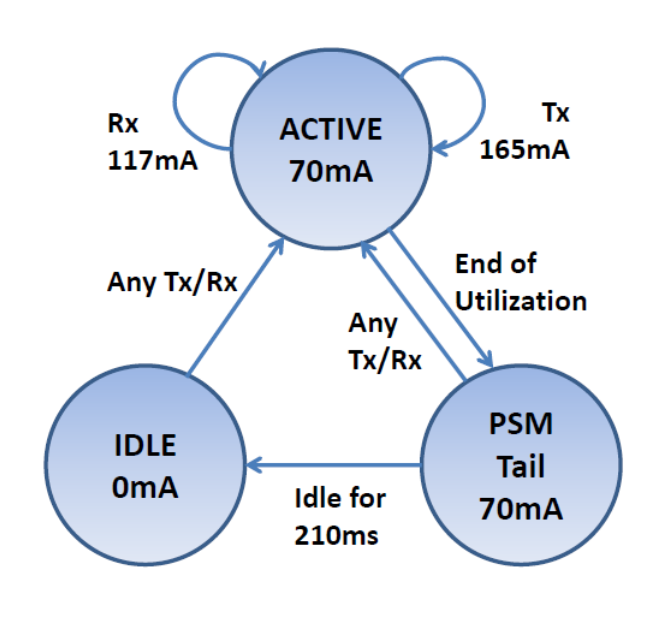
\includegraphics[width=0.4\textwidth]{figures/wifi_statemachine.png}
\caption{Typical power state-machine of a Wi-Fi antenna \cite{Ding:2013:CMI:2465529.2466586}}
\label{fig:hw:statemachine}
\vspace {-0.32in}
\end{figure}

\subsubsection{Monitoring the energy-state using the \batterystats{} 
history}

Based on the ideas in \cite{petra}, we initially looked at using the 
energy tools part of the Android Open Source Project. The 
\batterystats{} history contains a time-line of energy related events 
that occurred since last charge or reset. However, it was found that 
this history doesn't record the switches to the tail state. Hence, 
another approach was needed -- monitoring events which trigger these 
switches, namely network traffic events.

The Dalvik Debug Monitor Server (DDMS) provides tools to monitor the 
network traffic in real time for a given application \cite{ddmstrafic}. 
This meant that the raw data used by this tool was stored on the device 
and it was found that network statistics at the application level were 
stored located in the directory \texttt{proc/net/xt\_qtaguid/stats} 
\cite{netxtqtaguid}. This file contains one line per \texttt{(app\_uid, 
tag)} pair, describing the associated network traffic, as presented on 
Figure \ref{fig:hw:xtstats}.

A \python{} procedure was written to parse this file and to return a 
pair \texttt{(rx\_bytes, tx\_bytes)}, aggregating all the incoming and 
outgoing traffic induced by a given application. The command \texttt{adb 
shell cat} was used to fetch this file and the program was able to 
update the statistics once every 45ms. This program therefore had the 
potential to monitor the network traffic caused by an application with a 
sampling period of about 50ms. However, it would require to use an 
actual device as there is no Wi-Fi emulation on AVDs.

%Investigations were conducted to the improve sampling frequency of this 
%tool as tests have shown that most of the time was spent fetching the 
%raw data from the device and it was conjectured that most of this time 
%was spent establishing connection with the device. An attempt was made 
%to use the interactive mode of the \texttt{adb shell} command-line tool 
%in order to establish a long-lived connection. Unfortunately, it was 
%found that the data was not refreshed once the connection was 
%established and this approach didn't succeed.

\begin{figure}
\begin{lstlisting}
idx iface uid_tag_int cnt_set rx_bytes rx_packets tx_bytes tx_packets
2 wlan0 0 0 200888 1096 79636 888
3 wlan0 0 1 0 0 0 0
\end{lstlisting}
\caption{Extract of \texttt{proc/net/xt\_qtaguid/stats}}
\label{fig:hw:xtstats}
\vspace {-0.32in}
\end{figure}

\subsection{Implementation}

Using these findings, two pieces of software were implemented in order 
to correlate the routine calls with the Wi-Fi energy activity; (i) a 
\python{} script to log the switches between the various energy states 
of the Wi-Fi antenna, and (ii) an analyser to process this data and 
generate results interpretable by the user. A test application was also 
written to evaluate the quality of the results generated.

\subsubsection{Monitoring the Wi-Fi energy state}

Algorithm \ref{alg:netmonitor} shows the pseudo-code and it simply 
fetches the most up-to-date network data and compares it with the 
previous one. If this data has changed, it means that some network 
traffic was induced by the application and that the antenna just 
switched to the active mode. Otherwise, no traffic occurred and if the 
antenna was in the active mode, it switches to the tail mode and resets 
a counter indicating the time when the tail mode started. If the antenna 
was in the tail mode, the algorithm then uses this counter to compute 
how much time was spent in that mode and switches to the idle mode if 
needed. If the antenna was already in idle mode, it should remain in 
that mode. We also ensure that, despite the loss of precision due to the 
sampling period, the duration of the tail-mode is never longer than the 
tail-time specified by the transition condition in the state-machine.

Initially, the clock used to produce the timestamps of the state 
switches was the clock of the host machine. However, the timestamps of 
the messages logged by the instrumented application and pulled using 
\logcat{} are produced by the clock of the mobile device. In order to 
correlate the routine calls and the energy consumption of the Wi-Fi 
antenna, \Orka{} needs to merge-sort these two files and to replay the 
resulting log file. To accurately sort the timestamps, \Orka{} would 
need to synchronise the clock of the mobile device with the clock of the 
host machine. After some investigations, it was found that it is only 
possible to set the Android clock via the ADB with a precision of one 
second, which is too low for this study. Many networking protocols able 
to synchronise clocks are available in the literature, but most of them 
are quite complex to use and were discarded at first. As \Orka{} has to 
deal with the Android clock in the \logcat{} dump, this clock should 
also be used to timestamp the switches between the energy states. To 
this end, the host machine now opens the connection with the device and 
send two commands: the first one to get the epoch time and the second to 
fetch the file containing the network statistics.

The logs generated by the \texttt{networkMonitor} module, a typical 
output of which is presented in Figure \ref{fig:netstats}, will be 
referred to as the \netstats{} logs or traces. These results were 
compared with the ones produced by DDMS and it was found that the 
antenna was successful logged in active or tail mode when traffic was 
reported by DDMS. Moreover, the sampling period of \Orka{} is twice as 
small as the one of DDMS, as the smallest sampling period offered by 
this tool is 100ms.


\begin{algorithm}
\KwIn{Active ADB connection to an actual device}
\KwOut{Logs of the energy states of the Wi-Fi antenna}
Get first network statistics $S_0$ at current time $t_0$\;
$state \leftarrow \texttt{IDLE}$\;
\While{True}{
Get network statistics $S_1$ at current time $t_1$\;
\uIf{$S_0 \neq S_1$}
{$state \leftarrow \texttt{ACTIVE}$\;}
\ElseIf{state = \texttt{ACTIVE}}{$state \leftarrow \texttt{TAIL}$\;$tail_{start} \leftarrow t_0$\;}
\If{$state = \texttt{TAIL}$ {\normalfont \textbf{and}} $t_1 - tail_{start} \geq tail_{time}$}
{Log $(t_0, state)$\;
$t_0 \leftarrow tail_{start} + tail_{time}$\;
$state \leftarrow \texttt{IDLE}$\;}
Log $(t_0, state)$\;
$t_0 \leftarrow t_1$\;
$S_0 \leftarrow S_1$\;
}
\caption{Network monitor}
\label{alg:netmonitor}
\end{algorithm}

\begin{figure}
\begin{lstlisting}
1503657227.287407 ACTIVE
1503657227.323574 TAIL
1503657227.359771 TAIL
1503657227.394717 TAIL
1503657227.428777 ACTIVE
1503657227.467203 TAIL
1503657227.518874 ACTIVE
1503657227.589833 ACTIVE
1503657227.644556 TAIL
1503657227.681700 TAIL
1503657227.716493 TAIL
1503657227.753575 TAIL
1503657227.789498 TAIL
1503657227.829724 TAIL
1503657227.864556 IDLE
1503657227.882524 IDLE
\end{lstlisting}
\caption{Extract of a typical \netstats{} output}
\label{fig:netstats}
\vspace {-0.32in}
\end{figure}

\subsubsection{Analysing the traffic and execution traces}

Once the simulation terminates, \Orka{} needs to process this new data 
to compute the estimates modelling the tail-behaviour induced by each 
injected routine. To model this information, the \texttt{routine} class 
was extended to store how much time was spent by the Wi-Fi antenna in 
each energy state while the routine was executed.

The \texttt{routine} class now includes a dictionary mapping each energy 
state to the time spent in this state while the routine was executed. 
For instance, a routine executed for ten seconds without using the Wi-Fi 
will be modelled by the following dictionary: 
\texttt{\{\textquotesingle{}ACTIVE\textquotesingle{}: 0.0, 
\textquotesingle{}TAIL\textquotesingle{}: 
0.0,\textquotesingle{}IDLE\textquotesingle{}: 10.0\}}. The \logcat{} 
data is used to keep track of the call stack and the \netstats{} data to 
update the energy state of the Wi-Fi antenna. The main function simply 
parses the \logcat{} and \netstats{} traces and performs a merge sort of 
these two files in order to process the logs chronologically. For each 
new entry, the time elapsed in the current state since the last entry is 
added to all the methods in the call stack. The Wi-Fi state and the call 
stack are then updated accordingly with this new entry. Once the logs 
have been fully processed, the results, which include the tuples storing 
the time spent in each energy state for all the injected routines, are 
written to disk. A typical extract of these results is presented in 
Figure \ref{fig:tailfeedback}.

\begin{algorithm}[h]
\KwIn{\logcat{} and \netstats{} traces}
\KwOut{Energy tuples describing the Wi-Fi activity for each injected routine}
Initialise routine cost tuples\;
Initialise call stack\;
$state \leftarrow \texttt{IDLE}$\;
\While{{\normalfont Log files contain entries left to process}}{
Get the non-processed entry with the smallest time-stamp\;
Add time spent since the last update in the current state to all routines in the stack\;
Update the call stack if the entry comes from \logcat, otherwise update the $state$\;
}
\caption{Network analyser}
\label{alg:netanal}
\end{algorithm}

\begin{figure}
\begin{lstlisting}
MainActivity.<init> {'ACTIVE': 0.0, 'IDLE': 0.01100015640258789, 'TAIL': 0.0}
MainActivity$1.onCheckedChanged {'ACTIVE': 0.0, 'IDLE': 0.03099989891052246, 'TAIL': 0.0}
MainActivity$2.onClick {'ACTIVE': 0.0, 'IDLE': 0.01699995994567871, 'TAIL': 0.0}
MainActivity.onCreate {'ACTIVE': 0.0, 'IDLE': 0.13199996948242188, 'TAIL': 0.0}
MainActivity$SendGet.run {'ACTIVE': 1.5723857879638672, 'IDLE': 0.8458666801452637, 'TAIL': 1.626746654510498}
\end{lstlisting}
\caption{Extract of a typical output of the \texttt{networkAnalyser}}
\label{fig:tailfeedback}
\vspace {-0.32in}
\end{figure}

Building on these new modules, \Orka{} is now able to monitor the 
network traffic and to correlate the network activity with the routine 
calls. Specifically, \Orka{} is now able to know which routines produce 
network traffic and to attribute them the corresponding energy usage, 
while taking tail-energy into account. The evaluation conducted shows 
that the measurements produced by \Orka{} at the application level 
verify the high-level observations on tail energy.
